\documentclass{article}

\usepackage{microtype}
\usepackage{graphicx}
\usepackage{subcaption}
\usepackage{booktabs}
\usepackage{placeins}
\usepackage{hyperref}
\newcommand{\theHalgorithm}{\arabic{algorithm}}
\usepackage{icml2026}
\usepackage{iftex}
\ifXeTeX
  % Tectonic uses XeTeX.  Its legacy `times` package can otherwise fall back
  % to Latin Modern; TeX Gyre Termes is the metrically compatible Times face.
  \usepackage{fontspec}
  \setmainfont{texgyretermes}[
    Path=fonts/, Extension=.otf,
    UprightFont=*-regular, BoldFont=*-bold,
    ItalicFont=*-italic, BoldItalicFont=*-bolditalic]
  \setsansfont{texgyreheros}[
    Path=fonts/, Extension=.otf,
    UprightFont=*-regular, BoldFont=*-bold,
    ItalicFont=*-italic, BoldItalicFont=*-bolditalic]
  \setmonofont{texgyrecursor}[
    Path=fonts/, Extension=.otf,
    UprightFont=*-regular, BoldFont=*-bold,
    ItalicFont=*-italic, BoldItalicFont=*-bolditalic]
\fi
\usepackage{amsmath}
\usepackage{amssymb}
\usepackage{mathtools}
\usepackage{amsthm}
\usepackage[capitalize,noabbrev]{cleveref}

\theoremstyle{plain}
\newtheorem{proposition}{Proposition}[section]
\newtheorem{lemma}[proposition]{Lemma}
\theoremstyle{remark}
\newtheorem{remark}[proposition]{Remark}

\newcommand{\VerifiedModel}{Pythia-70M}
\newcommand{\VerifiedTensorCount}{6}
\newcommand{\VerifiedEvalTokens}{2,032}
\newcommand{\DensePPL}{71.3525}
\newcommand{\QLBytes}{3,248,832}
\newcommand{\QLNaturalBytes}{3,248,832}
\newcommand{\QLDeltaPPL}{6.762}
\newcommand{\StrictQSLNaturalBytes}{3,233,152}
\newcommand{\StrictQSLTailPaddingBytes}{15,680}
\newcommand{\StrictQSLDeltaPPL}{7.320}
\newcommand{\StrictQSLMinusQLPPL}{+0.558}
\newcommand{\RelaxedQSLExtraBytes}{5,056}
\newcommand{\RelaxedQSLDeltaPPL}{6.476}
\newcommand{\RelaxedQSLMinusQLPPL}{-0.286}
\newcommand{\StrictSLRho}{+0.030}
\newcommand{\StrictQSRho}{-0.423}
\newcommand{\StrictQLRho}{-0.572}
\newcommand{\ProxyCorrMin}{0.9970}
\newcommand{\ProxyCorrMax}{0.9995}
\newcommand{\OBSRecovery}{0.0269}
\newcommand{\OBSWins}{16/16}
\newcommand{\BlockRecovery}{0.0744}
\newcommand{\BlockExtraBytes}{82,944}
\newcommand{\StrictQSLWins}{4/16}

\newcommand{\ScalePilotJobCount}{3}
\newcommand{\ScalePilotSeed}{17}
\newcommand{\ScalePilotWindowCount}{8}
\newcommand{\ScalePilotEvalTokens}{1,016}
\newcommand{\ScalePilotNumericalSourceSHA}{\texttt{d5444b26c3f7}}
\newcommand{\ScalePilotPythiaSelectedTensors}{12}
\newcommand{\ScalePilotPythiaSelectedParams}{12,582,912}
\newcommand{\ScalePilotPythiaStrictMinusQLNLL}{+0.0054}
\newcommand{\ScalePilotPythiaStrictMinusQLPPL}{+0.609}
\newcommand{\ScalePilotPythiaStrictSLRho}{+0.026}
\newcommand{\ScalePilotPythiaStrictQSRho}{-0.334}
\newcommand{\ScalePilotPythiaStrictQLRho}{-0.588}
\newcommand{\ScalePilotPythiaStrictWins}{3/8}
\newcommand{\ScalePilotOPTSelectedTensors}{10}
\newcommand{\ScalePilotOPTSelectedParams}{23,592,960}
\newcommand{\ScalePilotOPTStrictMinusQLNLL}{+0.0009}
\newcommand{\ScalePilotOPTStrictMinusQLPPL}{+0.056}
\newcommand{\ScalePilotOPTStrictSLRho}{+0.087}
\newcommand{\ScalePilotOPTStrictQSRho}{-0.367}
\newcommand{\ScalePilotOPTStrictQLRho}{-0.611}
\newcommand{\ScalePilotOPTStrictWins}{5/8}
\newcommand{\ScalePilotQwenSelectedTensors}{10}
\newcommand{\ScalePilotQwenSelectedParams}{31,457,280}
\newcommand{\ScalePilotQwenStrictMinusQLNLL}{+0.0073}
\newcommand{\ScalePilotQwenStrictMinusQLPPL}{+0.222}
\newcommand{\ScalePilotQwenStrictSLRho}{+0.022}
\newcommand{\ScalePilotQwenStrictQSRho}{-0.521}
\newcommand{\ScalePilotQwenStrictQLRho}{-0.743}
\newcommand{\ScalePilotQwenStrictWins}{1/8}


\icmltitlerunning{Exact-Byte Compression}

\begin{document}

\twocolumn[
  \icmltitle{When Do Compression Errors Cooperate?\\
  Exact-Byte Hessian Geometry for Composite Language-Model Compression}

  \begin{icmlauthorlist}
    \icmlauthor{Anonymous Authors}{anon}
  \end{icmlauthorlist}
  \icmlaffiliation{anon}{Anonymous Institution}
  \icmlcorrespondingauthor{Anonymous Authors}{anonymous@example.com}
  \icmlkeywords{language-model compression, post-training quantization, pruning, low-rank repair, Hessian geometry, rate distortion}
  \vskip 0.3in
]

\printAffiliationsAndNotice{}

\begin{abstract}
Low-bit quantization, pruning, scale protection, and low-rank correction can each be benign for small perturbations, suggesting that distributing compression across mechanisms may avoid pushing any one beyond its local \emph{comfort zone}.  Testing this hypothesis is easy to bias because heterogeneous codecs carry different indices, factors, scales, descriptors, and alignment overhead.  We formulate composite post-training compression as a discrete exact-serialized-byte problem and decompose its local loss into gradient, self, cross, proxy-mismatch, and path-curvature terms in a declared positive-semidefinite geometry.  Our audited \VerifiedModel{} probe shows why orthogonality alone is insufficient: sparse and low-rank repairs are nearly orthogonal, yet a conservative component-scaled Q+S+L candidate loses to Q+L by \StrictQSLMinusQLPPL{} perplexity when tail-padded to the same \QLBytes{}-byte final file; its natural encoding leaves \StrictQSLTailPaddingBytes{} bytes unused.  Optimal Brain Surgeon (OBS) re-estimation meanwhile improves a fixed sparse payload at zero additional bytes.  Three separate seed-\ScalePilotSeed{} scalability-smoke jobs over Pythia-70M, OPT-125M, and Qwen3-0.6B repeat the near-orthogonal S--L geometry and the positive strict-QSL-minus-QL endpoint sign for similarly underfilled candidates, without being pooled or promoted to multi-seed evidence.  We release a round-trip research codec, loss-landscape probes, a fail-closed scale runner, and a training-dependence taxonomy separating frozen PTQ from backward-assisted and fine-tuned methods.
\end{abstract}

\section{Introduction}
\label{sec:introduction}

Weight-only post-training compression is no longer a single-knob problem.
Second-order quantizers, activation-aware scales, one-shot pruning, sparse
outliers, and low-rank error reconstruction all preserve different parts of a
pretrained model~\citep{frantar2023gptq,frantar2023sparsegpt,lin2024awq,dettmers2024spqr,zhang2024lqer}.
This diversity motivates a natural hypothesis: if every mechanism has a
small-perturbation regime in which loss grows slowly, then splitting a severe
compression target across several mechanisms could remain inside several
comfort zones and outperform concentrating all repair bytes in one mechanism
over the same mandatory quantized base.

Joint mechanisms and their interactions are not new by themselves.  SLiM
combines quantization, semi-structured sparsity, and low-rank compensation;
Harma et al. analyze Q/S order and non-orthogonality; OBR applies Hessian
compensation to joint quantization and sparsification; and prior rate--distortion
work couples Hessian or Fisher sensitivity to entropy or bit allocation
~\citep{mozaffari2025slim,harma2025effective,guo2026optimal,choi2017towards,orr2025optimal,young2025radio}.
We therefore study a narrower reproducibility question: what conclusions
survive when realized heterogeneous endpoints are decoded from a declared
self-describing artifact and compared by natural and final file bytes?

Two gaps obstruct a clean test.  First, a nominal bit rate does not determine a
heterogeneous artifact's size.  Sparse corrections need support indices and row
pointers; low-rank corrections need two factors; scales and codebooks need
descriptors; containers need headers and alignment.  A value-stream calculation
can therefore call two endpoints equal-rate even when their decoded files
differ.  Second, a small Hessian-weighted perturbation is not itself an
accuracy certificate.  The task Hessian may be indefinite, a PSD proxy may not
match it, the first-order term need not vanish, and curvature can drift along
the path to the final codec endpoint.

We study these gaps through \emph{exact-byte Hessian diagnostics}.  A
deterministic research codec serializes the selected tensors, round-trips every
endpoint, and charges codes, scales, sparse state, factors, descriptors, and
padding.  In a declared PSD activation-Gram geometry, realized Q, S, and L
increments are decomposed into self and signed cross terms.  A 13-point
interpolation then checks whether the local proxy tracks held-out NLL all the
way to the only deployable point, $\epsilon=1$.

Our contributions are:
\begin{itemize}
  \item an executable, byte-faithful protocol and fail-closed artifact
  validator, exact under the declared research codec, for
  quantization (Q), scale protection, sparse residuals (S), fixed-support
  Optimal Brain Surgeon (OBS)
  value repair, low-rank residuals (L), and their compositions;
  \item a theory that states what PSD near-orthogonality does guarantee and a
  stricter same-byte exchange condition that includes gradient, interactions,
  path error, and discrete byte overhead;
  \item a parameter-utilization analysis based on held-out loss recovered per
  added file byte, with zero-byte repairs reported separately; and
  \item an evidence-aware comparison framework separating data-free PTQ,
  calibrated frozen PTQ, backward-assisted correction, and global
  fine-tuning/quantization-aware training (QAT).
\end{itemize}

The current strict result is intentionally negative.  On one \VerifiedModel{}
run over \VerifiedTensorCount{} selected MLP tensors, Q+L and scaled Q+S+L are
both \QLBytes{} bytes, but their perplexity increases are \QLDeltaPPL{} and
\StrictQSLDeltaPPL{}.  This verified physical endpoint shows that a logical
payload estimate is insufficient for the operational comparison.  Its strict
QSL natural artifact is \StrictQSLTailPaddingBytes{} bytes below Q+L and is
tail-padded to equal final length, so this result rejects the tested
conservative per-layer candidate rather than a budget-exhausted global
frontier.  It does not establish that composite compression is universally
inferior.  We additionally
execute all native endpoints in three separate single-seed scalability-smoke
jobs: full Pythia-70M MLP scope and depth-stratified OPT-125M and Qwen3-0.6B
MLP scopes.  All three retain a positive strict-scaled-QSL-minus-QL NLL sign
despite near-orthogonal S--L proxy geometry.  This repeated diagnostic enlarges
the execution scope, but unequal tensor scopes and one seed preclude a pooled
or model-scale conclusion.

\section{Related Work and Comparison Lanes}
\label{sec:related}

\paragraph{Frozen post-training methods.}
GPTQ uses second-order information to update remaining weights during
quantization, while SparseGPT applies an analogous one-shot view to
pruning~\citep{frantar2023gptq,frantar2023sparsegpt}.  Wanda replaces the
second-order solve with an activation--magnitude score~\citep{sun2024wanda}.
AWQ searches activation-aware scales that protect salient
channels~\citep{lin2024awq}.  SpQR and SqueezeLLM combine dense low-bit state
with sparse high-precision state, but the latter's Fisher-sensitivity path
requires loss gradients and therefore belongs in a different compute
lane~\citep{dettmers2024spqr,kim2024squeezellm}.  LQER, QERA, EoRA, and SLiM
reconstruct compression error in low-rank or joint sparse/quantized
representations~\citep{zhang2024lqer,zhang2025qera,liu2024eora,mozaffari2025slim}.
OBR applies closed-form Hessian compensation to joint quantization and
sparsification~\citep{guo2026optimal}.  Optimal Brain Surgeon and Optimal
Brain Compression already establish the broader second-order correction
lineage~\citep{hassibi1993obs,frantar2022obc}.  Fixed-support OBS refitting,
low-rank reconstruction, and Q/S/L composition are therefore baselines and
mechanisms in this paper, not base novelty claims.

\paragraph{Interaction, orthogonality, and rate precedents.}
Harma et al. prove that magnitude sparsification and max-scaled quantization
are generally non-orthogonal and analyze their order-dependent compound
error~\citep{harma2025effective}.  Their transformation-level notion differs
from our signed, order-specific cross term under a common local PSD proxy, but
it precludes any claim that this paper is the first interaction or
orthogonality analysis.  ProjQ likewise coordinates quantization noise with a
low-rank adapter through orthogonal subspace projection~\citep{yu2026projq}.
Choi et al. combine Hessian-weighted distortion with Huffman coding and
entropy-constrained scalar quantization~\citep{choi2017towards}; Orr et al.
study variable-length weight formats and Fisher rate allocation
~\citep{orr2025optimal}; and Radio optimizes an LLM rate--distortion
objective~\citep{young2025radio}.  Our narrower target is an executable,
byte-faithful audit under a declared research codec: every compared endpoint
is round-trip decoded, its natural and padded file bytes are separated, and
its signed local-PSD interactions are checked against realized NLL.  This is
not a claim of the first Hessian-aware rate allocation or the first compressed
bitstream.

\paragraph{End-loss, adaptive, and trained recovery.}
GuidedQuant uses end-loss information and YAQA performs full-model adaptive
rounding; these works make
the evaluation objective more explicit but use different optimization
budgets~\citep{kim2025guidedquant,tseng2026yaqa}.
Q-Palette targets fractional-bit allocation with codebooks~\citep{lee2025qpalette}.
LiftQuant adds block correction and an optional end-to-end stage, while
FPTQuant learns function-preserving transformations~\citep{he2026liftquant,vanbreugel2026fptquant}.
SliderQuant learns fused channel scales and small low-rank auxiliary repairs
under local sliding-window reconstruction, making it a close lane-B analogue
to our scale-plus-low-rank parameter-utilization question~\citep{wang2026sliderquant}.
Recent low-rank residual methods further refine where error should be
preserved or reconstructed~\citep{cho2026srr,park2026serq,li2026rescomp}.
We keep data-free frozen, calibrated no-backward, backward-assisted, and
globally trained methods in separate lanes because these are different
experimental interventions.

\begin{table}[t]
  \caption{Training-dependence lanes used throughout the comparison.}
  \label{tab:lane-summary}
  \centering
  \small
  \begin{tabular}{@{}clp{4.2cm}@{}}
    \toprule
    Lane & Backward? & Intervention \\
    \midrule
    A0 & No & Data-free frozen compression \\
    A1 & No & Calibration-only frozen compression \\
    B  & Yes & Encoder-side gradient/Hessian--vector products (HVPs), no global recovery \\
    C  & Yes & Learned or globally fine-tuned recovery \\
    \bottomrule
  \end{tabular}
\end{table}

The selected primary-source protocol and payload audit is reported in
\cref{tab:lanes}.  It is a literature taxonomy, not a protocol-matched
empirical leaderboard.

\section{Exact-Byte Composite Compression}
\label{sec:method}

\paragraph{Scope and objective.}
Let $\mathcal{T}$ be an ordered manifest of eligible weight matrices and
$w_0$ their dense FP16 values.  A codec endpoint $z$ decodes to
$\widehat w(z)$ and has on-disk length $\mathcal{B}(z)$.  For a fixed
manifest, model, and held-out distribution, the discrete problem is
\begin{equation}
  \min_{z\in\mathcal{Z}}\;
  \mathcal{L}(\widehat w(z))
  \quad\text{s.t.}\quad \mathcal{B}(z)\le B.
  \label{eq:discrete-rate}
\end{equation}
The same $\mathcal{T}$ is used for every comparator; all other model weights
remain dense.  Thus bytes in this paper describe the selected-tensor artifact,
not a whole checkpoint or inference package.

\paragraph{Byte-faithful codec.}
For each tensor, the artifact stores packed signed Q codes, FP16 row or
row--column-block scales, optional FP16 sparse values with fixed-width
compressed sparse row (CSR)
support, and optional FP16 low-rank factors.  A deterministic manifest stores
shapes, dtypes, stream offsets, and alignment.  We report both natural bytes
and final file bytes after 64-byte alignment and tail padding, then verify file
length, SHA-256, decoding, and elementwise equality with the evaluated FP16
endpoint.  This is an auditable research format, not a claim of production
kernel support.

\paragraph{Candidate mechanisms.}
Q is symmetric row-wise 4-bit round-to-nearest quantization.  Block-scale
protection solves bounded row--column-block multipliers in the local PSD
metric and stores the resulting FP16 scales.  S selects a residual support by
Wanda-style activation--magnitude importance; a matched control stores the
naive residual values.  OBS then re-estimates values on the \emph{same}
support, replacing already-paid values without changing the artifact layout.
L applies a covariance-whitened SVD to the post-Q residual and stores two FP16
factors.  Component scales for Q/S/L are solved jointly and folded into their
existing FP16 state, so a zero-byte claim is accepted only after natural and
file-byte verification.  The verified legacy endpoints use the declared
Q$\rightarrow$S$\rightarrow$L construction order; the new unexecuted matrix
also exposes L$\rightarrow$S as an order ablation.  We call Q+L a
\emph{single repair over the mandatory Q
base}, and Q+S+L a composite repair; neither phrase means that Q is absent.

\paragraph{Implemented PSD proxy.}
For layer $j$, calibration activations define a covariance $C_j$ and
\begin{equation}
 \begin{aligned}
 q_j(\Delta W)
   &=\tfrac12\operatorname{tr}(\Delta W C_j\Delta W^\top),\\
 \rho_H(a,b)
   &=\frac{\sum_j\langle a_j,b_j\rangle_{C_j}}
   {\sqrt{\sum_j\|a_j\|_{C_j}^2\sum_j\|b_j\|_{C_j}^2}}.
 \end{aligned}
 \label{eq:implemented-proxy}
\end{equation}
The reported normalized cost is
$\sum_j\|\Delta W_j\|_{C_j}^2/
 \sum_j\|W_j\|_{C_j}^2$.  Each empirical Gram receives a
$10^{-5}$ mean-diagonal ridge.  Matrices with relative negative spectrum worse
than $10^{-7}$ fail; accepted float32 numerical error is repaired once, and an
eight-machine-epsilon target and the applied diagonal shift are recorded per
layer.  Damping and the repair are identity shifts, so the final spectral
lower bound is derived from one validated eigenspectrum instead of repeating
cubic audit decompositions.  Whitened fitting retains one separate cached
eigendecomposition used to construct its square-root maps.  The same
prepared $C_j$ is used by selection, OBS, endpoint costs, Gram terms, and
$\rho_H$.  Whitened SVD has a separately disclosed numerical fit metric
$\widetilde C_j$: eigenvalues below a configurable fraction of
$\lambda_{\max}(C_j)$ are floored before forming the square root and inverse
square root.  The runner records that fraction, the number of clipped
eigenvalues, and the resulting condition number per layer.  Every decoded
candidate is still scored in $C_j$; factorizer regularization is not silently
presented as the common scoring metric.
For the unexecuted large-model smoke, each residual fit uses a seeded
randomized SVD with four oversampling vectors and two power iterations; the
resolved solver is recorded per layer.  Full SVD remains an explicit
small-matrix control, so computational approximation is not hidden inside the
geometry ablation.

\paragraph{Discrete strict-rate selection.}
For each layer and target, we enumerate feasible low-rank ranks.  At each rank,
the largest CSR support fitting the requested serialized cap is constructed;
the candidate with minimum activation-Gram cost is retained.  The strict QSL
control uses that layer's Q+L artifact as its cap, reserves alignment slack,
and is rejected before NLL evaluation if the aggregate serialized file exceeds
the Q+L file.  This is a deterministic layerwise constrained search, not a
claim of global discrete optimality.  It yields an executable endpoint rather
than a fractional rank or value-only relaxation.  A relaxed QSL point is
reported separately to show the effect of the next discrete allocation step.
The new, unexecuted aggregate allocator removes the forced-composition condition:
each layer may select Q, Q+S$_{\rm OBS}$, Q+L, or an enumerated QSL state.  It
adds intermediate supports and 1.25/1.5/2.0 multiples of the local Q+L repair
allowance beyond base Q near the strongest rank states, thereby permitting
enumerated cross-layer byte borrowing.  It prunes an additive one-layer
byte/cost surrogate and checks every surviving combination with the exact
multi-layer serializer.  The additive pruning is heuristic; feasibility is
exact under the research codec, while optimality remains limited to this
enumerated budget-band state set.  We therefore do not call it a globally
optimal frontier.  Component scaling is fitted only after the unscaled QSL
allocation is selected, so the scaled row is a fixed-allocation post-selection
ablation rather than the optimum scaled candidate over the whole frontier.

\paragraph{Endpoint gate.}
For every retained endpoint, we evaluate
$w(\epsilon)=w_0+\epsilon(\widehat w-w_0)$ on held-out text at 13 fixed
values from 0 to 1.  The first five points through $\epsilon=1/8$ fit a local
linear--quadratic model; the full path measures proxy/NLL correlation.  Only
$\epsilon=1$ is serialized and eligible for a rate--accuracy conclusion.

\section{Theory and Diagnostic Predictions}
\label{sec:theory}

\paragraph{Curvature is not automatically a geometry.}
Let $\mathcal{L}(w)$ be held-out loss, $g=\nabla\mathcal{L}(w_0)$, and
$J_0=\nabla^2\mathcal{L}(w_0)$.  The task Hessian $J_0$ may be
indefinite, so $x^\top J_0x$ is not a squared norm and a ``Hessian
cosine'' based on it need not be an angle.  We reserve $H\succeq0$ for
a declared positive-semidefinite metric: an empirical Fisher, a
generalized Gauss--Newton matrix, the activation Gram proxy used in our
experiments, or $J_0+\lambda I$ only when $\lambda$ is large enough to
make it PSD.  We write
$\langle a,b\rangle_H=a^\top Hb$ and
$\|a\|_H^2=a^\top Ha$; zero-energy directions are excluded when a
correlation is reported.

\paragraph{Self, cross, and path terms.}
For sequential compression stages, define the realized increments
$\delta_i=w_i-w_{i-1}$ and $\delta=\sum_i\delta_i$.  This telescoping
identity is exact, although each $\delta_i$ depends on stage order.  A
local expansion around $w_0$ can be written
\begin{equation}
\label{eq:loss-decomposition}
\begin{split}
\mathcal{L}(w_0+\delta)-\mathcal{L}(w_0)
={}&g^\top\delta\\
&+\frac{1}{2}\sum_i q_i+\sum_{i<j}c_{ij}
+\varepsilon_H(\delta),\\
q_i={}&\|\delta_i\|_H^2,\\
c_{ij}={}&\langle\delta_i,\delta_j\rangle_H .
\end{split}
\end{equation}
Here $\varepsilon_H$ contains both the mismatch between $H$ and $J_0$
and curvature variation along the path.  If $H=J_0$ and the Hessian is
$M$-Lipschitz in the relevant trust region, then
$|\varepsilon_H(\delta)|\le M\|\delta\|_2^3/6$.
Thus a small quadratic cost alone does not justify dropping the
first-order term or evaluating only an interpolation point with
$\epsilon<1$.

\paragraph{What near-orthogonality guarantees.}
For $q_iq_j>0$, define
\begin{equation}
\rho_H(i,j)=\frac{c_{ij}}{\sqrt{q_iq_j}},\qquad
\mu=\max_{i\ne j}|\rho_H(i,j)|.
\end{equation}
For $k$ components in a common PSD metric,
\begin{equation}
\label{eq:coherence-bound}
\bigl(1-(k-1)\mu\bigr)\sum_iq_i
\le \Bigl\|\sum_i\delta_i\Bigr\|_H^2
\le \bigl(1+(k-1)\mu\bigr)\sum_iq_i,
\end{equation}
with a nontrivial lower bound when $(k-1)\mu<1$.
Consequently, near-zero $\rho_H(S,L)$ says that the sparse and low-rank
repair costs are approximately additive.  It does \emph{not} say that
their self costs are small, that either is orthogonal to quantization,
or that the combination beats a single codec.  Likewise,
$\rho_H<0$ is cancellation, not orthogonality.  Achieving prescribed
orthogonality further requires the repair degrees of freedom to span
the relevant $H$-moments and to remain feasible after coefficient
rounding and serialization (Appendix~\ref{app:theory-proofs}).

\paragraph{Comfort zones at a common rate.}
Let $s_i\ge0$ denote compression burden assigned to mechanism $i$ in a
continuous relaxation, and let $d_i(s_i)$ be its local loss cost after
its fixed codec charges have been paid.  If the $d_i$ are differentiable
and convex inside their comfort zones, an interior allocation solving
$\min\sum_i d_i(s_i)$ subject to $\sum_i s_i=S$ satisfies
\begin{equation}
\label{eq:kkt-comfort}
d_i'(s_i)=\lambda\quad(s_i>0),
\qquad d_i'(0^+)\ge\lambda\quad(s_i=0).
\end{equation}
This separable condition assumes that allocation-dependent interactions
are negligible or absorbed into the $d_i$; otherwise their partial
derivatives enter the KKT condition.
In particular, if a single mechanism $A$ carries all burden $S$ and
$d_A'(S)>d_B'(0^+)$, shifting a sufficiently small amount to $B$
reduces the relaxed cost.  This formalizes the comfort-zone intuition,
but ranks only local candidates: ranks, sparse groups, descriptors, and
alignment make the deployable problem discrete.

For a strict byte test, let $A$ be a realized reference endpoint at budget
$B$, $u$ the degradation needed to free bytes, and $r$ a repair.  A frontier
claim additionally requires $A$ to be the best eligible single-mechanism
endpoint under the same protocol.
For the realized candidate $C=A+u+r$, define
\begin{align}
P_A(u)&=\mathcal{L}(A+u)-\mathcal{L}(A),\nonumber\\
G_A(r)&=\mathcal{L}(A)-\mathcal{L}(A+r),\nonumber\\
\Gamma_A(u,r)&=\mathcal{L}(A+u+r)-\mathcal{L}(A+u)\nonumber\\
&\quad-\mathcal{L}(A+r)+\mathcal{L}(A).
\end{align}
Then the combination is better at the same rate whenever its actual
serialized length obeys $\mathcal{B}(C)\le\mathcal{B}(A)$ and
\begin{equation}
\label{eq:exact-exchange}
G_A(r)>P_A(u)+\Gamma_A(u,r).
\end{equation}
Locally, $\Gamma_A(u,r)$ contains the curvature cross term
$u^\top H_A r$ plus proxy and path errors, where $H_A$ is the declared
PSD proxy at $A$.  Equation~\eqref{eq:exact-exchange}, not pairwise
orthogonality, is the relevant sufficient condition.

\paragraph{Repair efficiency must charge the file.}
For a positive marginal file cost
$m_r=\mathcal{B}(A+r)-\mathcal{B}(A)$, we report
$\eta_{\mathrm{NLL}}=G_A(r)/m_r$.  The byte function includes codes,
scales, sparse values, indices and row pointers, low-rank factors,
descriptors, manifests, headers, and alignment/padding.  Parameter count or
value-only bits cannot substitute for this ledger.  If OBS value
re-estimation or a folded scale changes no final bytes, its direct
held-out recovery is reported separately rather than as infinite
efficiency; the zero-byte claim also requires decoding to contain no
hidden state.  A local quadratic ranking remains diagnostic until the
final decoded endpoint is evaluated on held-out data.

These distinctions first appeared in one seed on six selected Pythia-70M
MLP tensors: $S$ and $L$ are nearly orthogonal in the PSD proxy, both
correlate negatively with $Q$, and a conservative QSL candidate is
nevertheless worse than Q+L after tail padding to the same final bytes.  Three
additional, unpooled scalability-smoke jobs execute
the same diagnostic over full Pythia MLP scope and depth-stratified OPT and
Qwen MLP scopes.  They repeat the near-orthogonal S--L category and positive
strict-QSL-minus-QL endpoint sign for similarly underfilled candidates
(\cref{tab:scaling-pilot}), but they are
still single-seed observations with unequal scopes.  Multi-seed, common-scope,
multi-rate, and production-format tests remain confirmatory requirements.

\section{Experimental Protocol}
\label{sec:experiments}

\paragraph{Verified exploratory endpoint.}
The currently verified artifact uses the pinned Pythia-70M checkpoint
\citep{biderman2023pythia}, WikiText-2 raw validation text
\citep{merity2017wikitext}, and six MLP projections from the first,
middle, and last transformer blocks.  Calibration and evaluation source texts
are content-disjoint; fallback text is disabled.  Held-out metrics cover
\VerifiedEvalTokens{} next-token predictions and dense perplexity
\DensePPL{}.  The target selected-tensor artifact ratio is 0.258 relative to
an FP16 reference.  Six strategies are probed on 13-point paths, and 16 fixed
contiguous windows provide paired descriptive differences.  These windows are
not treated as independent population samples.

\paragraph{Completed scalability smoke.}
We execute every native endpoint once at seed \ScalePilotSeed{} and target
selected-weight artifact ratio 0.258 on three scopes.  Pythia-70M uses all
\ScalePilotPythiaSelectedTensors{} transformer-block MLP projections;
OPT-125M~\citep{zhang2022opt} uses \texttt{fc1/fc2} in five depth-stratified
blocks (\ScalePilotOPTSelectedTensors{} tensors); and
Qwen3-0.6B~\citep{yang2025qwen3} uses \texttt{up/down} projections
in five blocks, excluding its gate projection
(\ScalePilotQwenSelectedTensors{} tensors).  Every job evaluates
\ScalePilotEvalTokens{} next-token predictions in eight fixed windows and
probes six directions on the same 13-point path.  All three share numerical
source \ScalePilotNumericalSourceSHA{}, record a per-layer PSD covariance
audit, and pass round-trip SHA and exact-file-byte checks.  The jobs are three
separate observations: each uses WikiText-2 raw validation text with
content-disjoint calibration/evaluation source windows and fallback disabled;
tokenizers and tensor scopes differ, and no cross-model metric is pooled or
ranked.

\paragraph{Preregistered and planned scale matrix.}
The released 69-job configuration also declares Pythia-160M/410M and
Llama-3.2-1B~\citep{grattafiori2024llama3}, multiple rates, and additional
seeds.  Those rows remain unexecuted.  Moreover, the present runner's seed
argument does not alter its sequential data windows, so repeated invocations
cannot be treated as independent confirmation.  The separate eight-seed
content-disjoint split manifest is preregistered but not yet consumed by this
runner.

\paragraph{Baselines and fairness.}
Native comparisons include Q, global and block scales, Q+S, Q+S with OBS,
Q+L, strict and relaxed QSL, Q+S$_{\rm OBS}$+L, and component-scaled QSL.
External methods enter a numeric table only if model checkpoint, W-only scope,
tensor manifest, calibration/evaluation data, and exported physical payload
match.  We report data-free A0, calibrated no-backward A1, local
backward-assisted B, and global fine-tuned/QAT C methods separately
(\cref{tab:lane-summary,tab:lanes}).  Literature numbers never populate
measured cells.

\paragraph{Metrics.}
Primary metrics are final file bytes, held-out NLL and perplexity change,
normalized PSD proxy cost, and all pairwise signed $\rho_H$.  For a positive
byte increment we use held-out NLL recovery per added byte.  Equal-byte
re-estimation is reported as direct recovery, not infinite efficiency.
Natural bytes, alignment, encoder wall time, peak memory, and provenance are
secondary diagnostics.

\section{Results and Analysis}
\label{sec:results}

\subsection{Physical accounting exposes the strict disadvantage}

\begin{table*}[t]
  \caption{Verified selected-tensor endpoints at target ratio 0.258.
  Scope: \VerifiedModel{}, six MLP linear tensors, one seed, and
  \VerifiedEvalTokens{} held-out tokens.  ``Natural'' precedes final tail
  padding; ``Final'' is the complete research artifact whose stream offsets
  use 64-byte alignment.  Lower
  $\Delta$NLL/$\Delta$PPL is better.}
  \label{tab:exact-rate}
  \centering
  \begin{tabular}{lrrrrr}
\toprule
Endpoint & Natural B & Final B & $\Delta$NLL & $\Delta$PPL & norm. $H$ \\
\midrule
Q & 3,167,552 & 3,167,552 & +0.1982 & +15.644 & 0.01008 \\
Q + block scale & 3,250,496 & 3,250,496 & +0.1238 & +9.404 & 0.00577 \\
Q+S & 3,260,546 & 3,260,546 & +0.1224 & +9.293 & 0.00680 \\
Q+S (OBS) & 3,260,546 & 3,260,546 & +0.0956 & +7.156 & 0.00586 \\
\textbf{Q+L} & \textbf{3,248,832} & \textbf{3,248,832} & \textbf{+0.0905} & \textbf{+6.762} & \textbf{0.00463} \\
Q+S+L, strict & 3,233,152 & 3,248,832 & +0.0977 & +7.320 & 0.00507 \\
Q+S+L, +5{,}056 B & 3,253,888 & 3,253,888 & +0.0869 & +6.476 & 0.00457 \\
\bottomrule
\end{tabular}

\end{table*}

\cref{tab:exact-rate} gives selected bounded endpoints; the complete native
method set is retained in the released CSV.  Q+L and strict component-scaled
QSL are both \QLBytes{} bytes, but strict component-scaled QSL is
\StrictQSLMinusQLPPL{} perplexity worse.  Its natural file is
\StrictQSLNaturalBytes{} bytes and receives \StrictQSLTailPaddingBytes{} bytes
of tail padding to match the \QLNaturalBytes{}-byte Q+L file.  The control is
therefore a feasible but under-filled, per-layer-guarded candidate rather than
a budget-exhausted global frontier.  Equal padded length prevents an overrun;
it does not prove optimal use of the available natural bytes.  The relaxed QSL endpoint
adds only \RelaxedQSLExtraBytes{} bytes and is
\RelaxedQSLMinusQLPPL{} perplexity relative to Q+L, but its paired interval
crosses zero.  This is evidence of a discrete threshold, not a confirmed
frontier improvement.

\begin{figure*}[t]
  \centering
  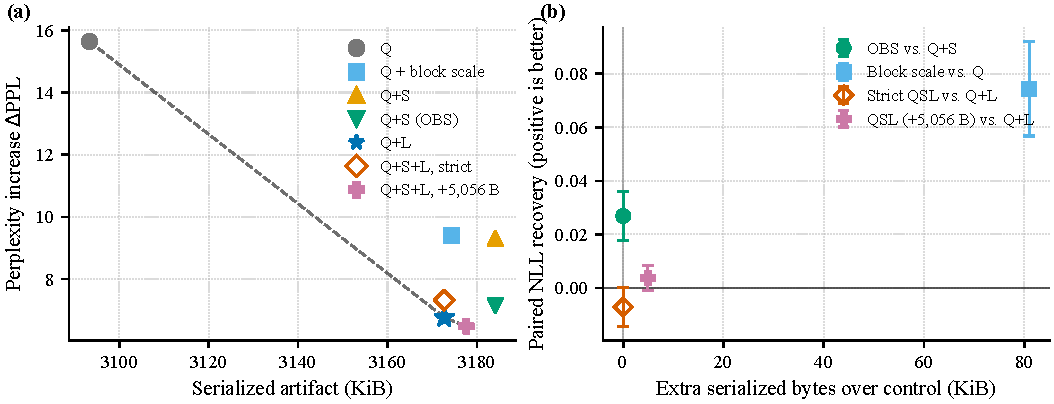
\includegraphics[width=0.98\textwidth]{figures/exact_rate_tradeoffs.pdf}
  \caption{Verified exact-rate trade-offs from committed CSV artifacts.
  (a) Physical bytes versus perplexity increase; only measured artifact files
  are plotted.  (b) Paired held-out NLL recovery and byte overhead for targeted
  repairs.  Error bars are descriptive normal intervals over 16 fixed windows,
  not population confidence intervals.  Scope is one seed and six selected
  Pythia-70M MLP tensors.}
  \label{fig:tradeoff}
\end{figure*}

\subsection{Which small parameters are used effectively?}

\begin{table}[t]
  \caption{Paired repair effects in the same bounded run.  Positive recovery
  favors the left method.  Intervals are descriptive over fixed windows.}
  \label{tab:repairs}
  \centering
  \resizebox{\columnwidth}{!}{\begin{tabular}{lrrrr}
\toprule
Comparison & $\Delta$ bytes & NLL recovery & 95\% interval & Wins \\
\midrule
OBS vs. Q+S & +0 & +0.0269 & [+0.0176, +0.0361] & 16/16 \\
Block scale vs. Q & +82,944 & +0.0744 & [+0.0568, +0.0921] & 16/16 \\
Strict QSL vs. Q+L & +0 & -0.0071 & [-0.0144, +0.0001] & 4/16 \\
QSL (+5{,}056 B) vs. Q+L & +5,056 & +0.0037 & [-0.0010, +0.0083] & 10/16 \\
\bottomrule
\end{tabular}
}
\end{table}

OBS is the clearest parameter-utilization result
(\cref{tab:repairs,fig:tradeoff}): it recovers \OBSRecovery{} mean NLL on an
unchanged support/value payload and improves \OBSWins{} windows.  It therefore
spends computation to make already-stored sparse values satisfy a local
stationarity condition.  Block scales recover \BlockRecovery{} NLL on all
  windows, but require \BlockExtraBytes{} additional bytes.  Q+L recovers more
  NLL per added byte than block scales in this tensor shape; the measured
  low-rank direction fits this residual more effectively, but one run does not
  establish a causal architectural advantage.  The strict QSL exchange instead
removes useful rank/support capacity to pay discrete sparse metadata and the
legacy per-layer alignment guard, and wins
only \StrictQSLWins{} windows against Q+L.

This suggests an analogue of scale protection for pruning: freeze a small
support, then optimize its values (OBS) rather than buying more survivors.
More generally, a repair is attractive when it changes existing stored state,
spans a high-energy residual direction, and avoids a new descriptor or index
threshold.

\subsection{Near-orthogonality is not sufficient}

At the strict endpoint,
$\rho_H(S,L)=\StrictSLRho{}$, but
$\rho_H(Q,S)=\StrictQSRho{}$ and
$\rho_H(Q,L)=\StrictQLRho{}$ (\cref{fig:geometry}).  S and L are nearly
orthogonal to each other; both cancel part of Q.  The three-way perturbation is
not mutually orthogonal, and the small S--L cross term cannot compensate for
their self costs or the capacity sacrificed to fit strict bytes.  This is the
observed counterpart of \cref{eq:exact-exchange}.

\begin{figure*}[t]
  \centering
  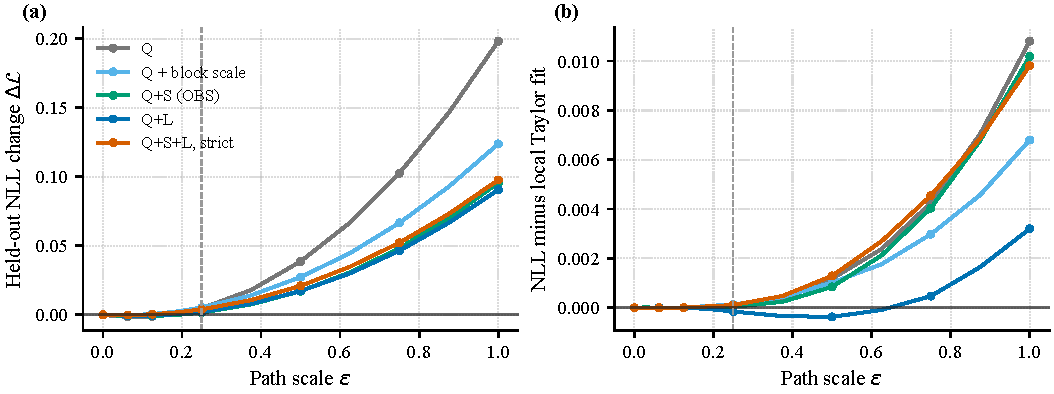
\includegraphics[width=0.98\textwidth]{figures/loss_landscape.pdf}
  \caption{Held-out loss landscapes for six codec directions in the original
  bounded probe.  Left: NLL along the 13-point interpolation.  Right: residual
  after the local linear--quadratic fit.  Proxy/path correlations range from
  \ProxyCorrMin{} to \ProxyCorrMax{}, yet nonzero linear terms and endpoint
  residuals require final NLL evaluation.  Scope is one seed, six selected
  Pythia-70M MLP tensors, and \VerifiedEvalTokens{} held-out tokens.}
  \label{fig:landscape}
\end{figure*}

The activation-Gram proxy tracks these particular paths closely
(\cref{fig:landscape}), but every fitted linear coefficient is negative.
Consequently, comparing only $\delta^\top H\delta$ omits a measurable
first-order contribution.  High correlation supports radial quadratic shape
only along each already selected direction; it does not validate cross-candidate
ranking and is not a certificate outside those directions or across models.

\subsection{Three scalability-smoke observations}

\begin{table*}[t]
\centering
\caption{Single-seed scalability smoke at target selected-weight artifact ratio 0.258. Pythia covers all MLP projections, while OPT and Qwen use ten depth-stratified MLP projections. Bytes are complete aligned research-codec files for selected tensors, not whole-model or production payloads. ``Strict$-$QL'' is the signed held-out NLL difference after tail padding to identical final bytes; the strict natural files leave 31,360/640/1,024 bytes unused for Pythia/OPT/Qwen. Negative favors the composite. Rows are not pooled or ranked across models.}
\label{tab:scaling-pilot}
\footnotesize
\setlength{\tabcolsep}{4.5pt}
\begin{tabular*}{\textwidth}{@{\extracolsep{\fill}}lrrrrrrr@{}}
\toprule
Model / scope & \shortstack{Tensors /\\M params} & \shortstack{QL=strict\\bytes (rate)} & $\Delta$NLL QL & $\Delta$NLL strict & Strict$-$QL & $\rho_{SL}$ & $\rho_{QS}/\rho_{QL}$ \\
\midrule
Pythia-70M / full MLP & 12 / 12.58 & 6,497,344 (0.2581) & +0.1963 & +0.2017 & +0.0054 & +0.026 & -0.334/-0.588 \\
OPT-125M / 5-depth MLP & 10 / 23.59 & 12,158,976 (0.2577) & +0.0735 & +0.0744 & +0.0009 & +0.087 & -0.367/-0.611 \\
Qwen3-0.6B / 5-depth MLP & 10 / 31.46 & 16,196,352 (0.2574) & +0.0226 & +0.0299 & +0.0073 & +0.022 & -0.521/-0.743 \\
\bottomrule
\end{tabular*}
\end{table*}


\begin{figure*}[t]
  \centering
  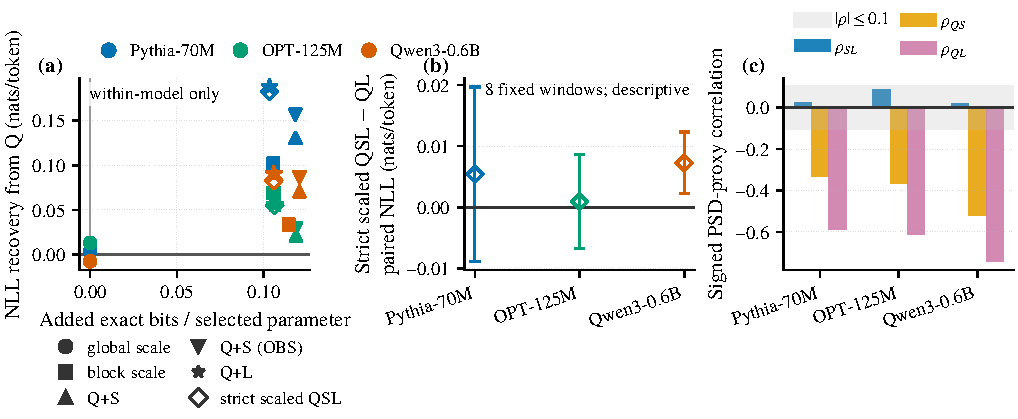
\includegraphics[width=0.99\textwidth]{figures/scaling_pilot_efficiency_geometry.pdf}
  \caption{Mechanism behavior in three separate seed-\ScalePilotSeed{}
  scalability-smoke jobs.  (a) Within each color/model, held-out NLL recovery
  from Q versus added exact file bits per selected parameter; the zero-byte
  scale point is direct folded re-estimation, not infinite efficiency.
  (b) Conservative strict component-scaled QSL minus Q+L after tail padding
  to identical final file bytes; the strict natural files underfill their Q+L
  caps by 31,360, 640, and 1,024 bytes for Pythia, OPT, and Qwen, respectively;
  error bars are descriptive mean $\pm1.96$ sample standard errors over eight
  fixed windows, not confidence intervals or significance tests.  (c) Signed
  activation-Gram correlations; the band marks $|\rho|\le0.1$, while negative
  Q--S/Q--L values denote cancellation.  Tokenizers and tensor scopes differ,
  so magnitudes are not ranked across models and rates are not whole-model
  compression ratios.}
  \label{fig:scaling-smoke}
\end{figure*}

The strict scaled composite is higher-NLL than Q+L in all three decoded,
final-byte-equal but naturally underfilled endpoints: by
\ScalePilotPythiaStrictMinusQLNLL{} on Pythia,
\ScalePilotOPTStrictMinusQLNLL{} on OPT, and
\ScalePilotQwenStrictMinusQLNLL{} on Qwen.  The fixed-window descriptive
interval crosses zero for Pythia and OPT; Qwen favors Q+L in seven of eight
windows and its interval remains positive.  At the same time,
$\rho_H(S,L)$ is \ScalePilotPythiaStrictSLRho{},
\ScalePilotOPTStrictSLRho{}, and \ScalePilotQwenStrictSLRho{}, respectively,
whereas every Q--S and Q--L correlation is negative
(\cref{tab:scaling-pilot,fig:scaling-smoke}).  Thus the coherence diagnostic
remains compatible with local S--L additivity, but the realized exchange
condition in \cref{eq:exact-exchange} fails for each tested conservative
endpoint.  Because unused natural bytes were not reallocated across layers,
these observations do not reject every budget-exhausted composite.

The parameter-utilization controls are more mechanism-specific.  Block scales
improve Q in every job while paying positive descriptor/scale bytes, and OBS
value re-estimation improves Q+S in all three without changing the sparse file.
Folded global-scale re-estimation helps Pythia and OPT but hurts Qwen at the
same bytes.  This is precisely why zero-byte state reuse is attractive yet
still requires held-out endpoint validation: low parameter cost does not imply
a universally beneficial update.  The committed CSVs contain all 33 endpoints
and 234 path points.  The appendix tabulates every endpoint and visualizes the
78 Q+L/strict path points in
\cref{tab:scaling-pilot-all-endpoints,fig:scaling-paths}; none is collapsed
into a cross-model mean.

\subsection{What would establish a combination advantage?}

None of the current tail-padded strict candidates does relative to Q+L; OPT also contains
a lower-NLL, slightly smaller Q+block-scale endpoint.  A convincing positive
result at the same
compression rate must (i) use an identical tensor manifest and actual bytes,
(ii) keep each component's self cost in its low-curvature regime, (iii) control
all signed cross terms without calling cancellation orthogonality, (iv) clear
the discrete rank/support/descriptor threshold, and (v) retain a positive
held-out endpoint gain after the byte exchange.  In the notation of
\cref{eq:exact-exchange}, these requirements reduce to an executable
$G_A(r)>P_A(u)+\Gamma_A(u,r)$ test.  The new global allocator and large-model
method-ablation matrix are designed to test that inequality while allowing Q,
Q+S$_{\rm OBS}$, and Q+L as nested degenerate states.  Until those jobs
complete, they remain planned and are not silently promoted to results.

\FloatBarrier
\section{Limitations and Conclusion}
\label{sec:conclusion}

The strongest detailed probe remains one seed on six selected Pythia-70M
tensors, now accompanied by three separate seed-17 scalability-smoke jobs over
full Pythia MLP and depth-stratified OPT/Qwen MLP scopes.  Their repeated sign
is not multi-seed confirmation: the activation Gram is a PSD reconstruction
proxy rather than the task Hessian, fixed windows do not support population
inference, and unequal scopes forbid a model-scale trend.  The research codec
also does not establish kernel speed, whole-checkpoint size, or energy savings.
External methods remain literature-reported until their training budgets and
physical payloads are reproduced under a matched protocol.

Within that boundary, the result is consistent across the executed scopes:
sparse and low-rank repairs can be nearly orthogonal without a same-byte
composite advantage.  Exact serialization reveals the discrete cost that
logical accounting hides.  OBS improves the already-paid sparse payload in all
three smoke jobs, whereas zero-byte global-scale re-estimation has mixed sign;
parameter thrift therefore helps only when the fitted update also lowers the
held-out endpoint.  Composite compression is most plausible when mechanisms
exchange real bytes at favorable held-out marginal cost.  Orthogonality is one
diagnostic in that decision, not the decision itself.


\FloatBarrier
\section*{Impact Statement}
This work aims to make language-model compression comparisons more reproducible by charging actual serialized state and by separating diagnostic proxies from held-out endpoint evidence.  Better compression can reduce storage and inference-resource requirements, but accuracy losses can be uneven across tasks or populations.  The research artifact codec is not a production runtime, and the present experiments do not establish deployment speed, energy savings, safety preservation, or fairness preservation; those properties require separate evaluation before use.

\clearpage
\bibliography{references}
\bibliographystyle{icml2026}

\clearpage
\appendix
\section{Proofs and Scope of the Curvature Analysis}
\label{app:theory-proofs}

\subsection{Taylor expansion and the role of a PSD proxy}

Let $\mathcal{L}:\mathbb{R}^p\rightarrow\mathbb{R}$ be twice
continuously differentiable on the segment from $w_0$ to
$w_0+\delta$.  With $J(w)=\nabla^2\mathcal{L}(w)$, Taylor's integral
form gives
\begin{equation}
\label{eq:integral-taylor}
\mathcal{L}(w_0+\delta)-\mathcal{L}(w_0)
=g^\top\delta+
\int_0^1(1-t)\,\delta^\top J(w_0+t\delta)\delta\,dt.
\end{equation}
Writing $J_0=J(w_0)$ yields the usual quadratic term and a path
remainder.  If
$\|J(w_0+t\delta)-J_0\|_{\mathrm{op}}\le Mt\|\delta\|_2$, then
\begin{equation}
\left|\mathcal{L}(w_0+\delta)-\mathcal{L}(w_0)
-g^\top\delta-\tfrac12\delta^\top J_0\delta\right|
\le \frac{M}{6}\|\delta\|_2^3,
\end{equation}
because $\int_0^1t(1-t)dt=1/6$.

The task Hessian $J_0$ can be indefinite.  For geometric diagnostics we
instead select and disclose $H\succeq0$.  Combining proxy mismatch and
path variation gives
\begin{equation}
\label{eq:proxy-error-bound}
\begin{split}
\varepsilon_H(\delta)
={}&\tfrac12\delta^\top(J_0-H)\delta+R_3(\delta),\\
|\varepsilon_H(\delta)|
\le{}&\tfrac12\|J_0-H\|_{\mathrm{op}}\|\delta\|_2^2\\
&+\tfrac{M}{6}\|\delta\|_2^3.
\end{split}
\end{equation}
The bound need not be numerically tight; its purpose is to expose the
assumption hidden when a PSD surrogate is called ``the Hessian.''  For
a damped task Hessian, $H=J_0+\lambda I$ is a metric only when
$\lambda\ge-\lambda_{\min}(J_0)$.  Damping must therefore be reported,
and it changes the measured angles.  If $H$ is singular, its inner
product is understood on the quotient by $\ker(H)$; correlations with
$q_i=0$ are undefined rather than zero.

For sequential maps $T_1,\ldots,T_k$, let
$w_i=T_i(w_{i-1})$ and $\delta_i=w_i-w_{i-1}$.  Then
$w_k-w_0=\sum_i\delta_i$, so substituting into the $H$-quadratic gives
\begin{equation}
\frac12\Bigl\|\sum_i\delta_i\Bigr\|_H^2
=\frac12\sum_i\|\delta_i\|_H^2
+\sum_{i<j}\langle\delta_i,\delta_j\rangle_H.
\end{equation}
This algebra does not make the components order invariant.  If
$T_iT_j(w)\ne T_jT_i(w)$, changing order changes both increments and
the final endpoint; all terms must be recomputed after final decoding.

\subsection{Coherence bound}

\paragraph{Proposition 1 (PSD coherence).}
Let $H\succeq0$, let $q_i=\|\delta_i\|_H^2>0$, and suppose
$|\rho_H(i,j)|\le\mu$ for every $i\ne j$.  Then
Equation~\eqref{eq:coherence-bound} holds.

\paragraph{Proof.}
Cauchy--Schwarz in the PSD seminorm gives
$|\langle\delta_i,\delta_j\rangle_H|
\le\mu\sqrt{q_iq_j}$.  Moreover,
\begin{equation}
2\sum_{i<j}\sqrt{q_iq_j}
=\left(\sum_i\sqrt{q_i}\right)^2-\sum_iq_i
\le(k-1)\sum_iq_i,
\end{equation}
where the last inequality follows from
$(\sum_i\sqrt{q_i})^2\le k\sum_iq_i$.  Applying the upper and lower
signs to the cross-term expansion proves the claim. \hfill$\square$

The proposition controls only additivity of the PSD quadratic.  It
does not control $g^\top\delta$, proxy error, path remainder, component
self costs, or serialized rate.  A negative correlation may reduce the
quadratic through cancellation, but $|\rho_H|$ is then large and the
components are not near-orthogonal.

\subsection{Feasibility of enforced orthogonality}

Suppose an error $e$ can be modified using columns
$B=[b_1,\ldots,b_d]$ and we want the result to be $H$-orthogonal to
columns $U=[u_1,\ldots,u_m]$.  A coefficient vector $\alpha$ must solve
\begin{equation}
\label{eq:orthogonal-feasibility}
A\alpha=-c,\qquad A=U^\top HB,\qquad c=U^\top He.
\end{equation}
An unconstrained solution exists if and only if $-c$ lies in the range
of $A$.  Thus a single global scale generally cannot remove several
independent moments.  Codec feasibility adds stronger conditions:
$\alpha$ must respect the allowed scale range, support or rank, storage
precision, and descriptor layout.  After rounding, the residual
$\|A\widehat\alpha+c\|$ must be remeasured.  Subsequent requantization,
support selection, or rank truncation can reintroduce the moments, so
orthogonality is a property of the final decoded endpoint, not of an
intermediate floating-point solve.

\subsection{A sufficient endpoint comparison}

Define the local PSD score
\begin{equation}
\widehat\Delta_H(z)=g^\top z+\tfrac12 z^\top Hz
\end{equation}
and suppose a candidate-specific certificate satisfies
\begin{equation}
\left|\mathcal{L}(w_0+z)-\mathcal{L}(w_0)
-\widehat\Delta_H(z)\right|\le r(z).
\end{equation}
The radius $r(z)$ must include proxy mismatch and path curvature; it may
be estimated conservatively from held-out interpolation diagnostics but
is not supplied by coherence alone.

\paragraph{Proposition 2 (same-byte sufficient condition).}
Let $z_C$ be a composite candidate and $\{z_j\}$ the eligible
single-mechanism candidates.  If
\begin{equation}
\label{eq:certified-comparison}
\begin{split}
\mathcal{B}(z_C)&\le B,\\
\widehat\Delta_H(z_C)+r(z_C)
&<\min_{j:\,\mathcal{B}(z_j)\le B}
  \bigl\{\widehat\Delta_H(z_j)-r(z_j)\bigr\}.
\end{split}
\end{equation}
then the composite has lower loss than every eligible single candidate
at budget $B$.

\paragraph{Proof.}
The left side of the strict inequality upper-bounds the composite loss
increment, while every term on the right lower-bounds the corresponding
single-candidate increment. \hfill$\square$

This proposition is deliberately sufficient, not necessary.  In the
absence of a trustworthy $r(z)$, held-out endpoint loss replaces the
certificate; a high proxy/path correlation is a diagnostic, not a
proof of the inequality.

\subsection{Comfort-zone allocation}

Let each $d_i:[0,S]\rightarrow\mathbb{R}$ be differentiable, convex,
and nondecreasing in assigned compression burden.  Consider
\begin{equation}
\label{eq:continuous-allocation}
\min_{s_i\ge0}\sum_{i=1}^k d_i(s_i)
\quad\text{subject to}\quad \sum_{i=1}^k s_i=S.
\end{equation}

\paragraph{Proposition 3 (marginal-cost allocation).}
At an optimum of Equation~\eqref{eq:continuous-allocation}, every
active component satisfies $d_i'(s_i)=\lambda$ and every inactive
component satisfies $d_i'(0^+)\ge\lambda$.  If the all-$A$ allocation
has $d_A'(S)>d_B'(0^+)$ and both derivatives are continuous near the
endpoint, then an allocation using both $A$ and $B$ has strictly lower
cost.

\paragraph{Proof.}
The KKT stationarity and complementary-slackness conditions are
\begin{equation*}
d_i'(s_i)-\lambda-\nu_i=0,\qquad
\nu_i\ge0,\qquad \nu_i s_i=0.
\end{equation*}
They give the stated active and inactive conditions.  For the second
claim, set $f(\epsilon)=d_A(S-\epsilon)+d_B(\epsilon)$.  Then
$f'(0^+)=-d_A'(S)+d_B'(0^+)<0$, so sufficiently small positive
$\epsilon$ improves the objective. \hfill$\square$

Separability is an assumption of Equation~\eqref{eq:continuous-allocation}.
For an objective $\sum_i d_i(s_i)+\gamma(s)$ with non-negligible
allocation-dependent interactions, the active condition becomes
$d_i'(s_i)+\partial_i\gamma(s)=\lambda$.

The proposition explains why several mechanisms can outperform one
mechanism pushed beyond its comfortable region, but only in the stated
continuous model.  A codec has a lattice of feasible endpoints: one
rank, one sparse group, or a new descriptor may have a fixed charge.
The deployable analogue is a finite exact-byte exchange.

Let $A$ be a realized endpoint, $u$ a perturbation that frees payload,
and $r$ a repair perturbation.  For a fixed, order-specific decomposition
$C=A+u+r$, direct addition and subtraction gives
\begin{equation}
\label{eq:exchange-identity}
\mathcal{L}(C)-\mathcal{L}(A)=P_A(u)-G_A(r)+\Gamma_A(u,r).
\end{equation}
Hence Equation~\eqref{eq:exact-exchange} is equivalent to a strict
improvement once $\mathcal{B}(C)\le\mathcal{B}(A)$.  Around $A$, the
second-order part of $\Gamma_A$ is $u^\top J_A r$; replacing $J_A$ by a
PSD proxy again adds a mismatch and path term.  This identity also shows
why repair-to-repair orthogonality is insufficient: the cost of freeing
bytes and all interactions still remain.

\subsection{Physical bytes and parameter utilization}

For endpoint $z$, the comparison rate is the on-disk length
\begin{equation}
\label{eq:byte-ledger}
\begin{split}
\mathcal{B}(z)={}&B_{\rm header}+B_{\rm manifest}+B_{\rm descriptor}\\
&+B_{\rm codes}+B_{\rm scales}\\
&+B_{\rm sparse\ values}+B_{\rm indices}\\
&+B_{\rm rowptr}+B_{\rm factors}+B_{\rm alignment}\\
&+B_{\rm tail\ padding}.
\end{split}
\end{equation}
The marginal cost $m_r=\mathcal{B}(A+r)-\mathcal{B}(A)$ is therefore
integer-valued and need not equal the sum of value streams.  Alignment
can make it nonadditive.  We disclose both natural bytes and final file
bytes: the latter decides the strict budget, while the former reveals
when a nominally zero-cost change merely consumes padding slack.

When $m_r>0$, held-out recovery per byte is
\begin{equation}
\eta_{\rm NLL}(r\mid A)
=\frac{\mathcal{L}(A)-\mathcal{L}(A+r)}{m_r}.
\end{equation}
Suppose $u$ frees $f_u>0$ bytes and has loss penalty
$P_A(u)=f_u\eta_{\rm giveup}$.  If the repair has
$G_A(r)=m_r\eta_{\rm repair}$, then a feasible exchange improves loss
when
\begin{equation}
m_r\eta_{\rm repair}
>f_u\eta_{\rm giveup}+\Gamma_A(u,r),
\qquad m_r\le f_u,
\end{equation}
with any remaining slack represented in the actual serialization.
For an exactly matched exchange $m_r=f_u$, this reduces to an efficiency
comparison corrected by interaction per byte.  Merely comparing the two
ratios is not sufficient when the exchanged byte amounts differ.

If $m_r=0$, division would create an artificial infinite efficiency.
Instead we report the direct recovery, verify that the decoded artifact
contains no side state, and state whether natural bytes or only final
file bytes are unchanged.  Fixed-support OBS can satisfy this condition
when re-estimated values replace already stored values; a scale can do
so only if it is demonstrably folded into an already stored field.

\subsection{Limits of the diagnostic}

The analysis is local and order specific.  Its strongest threats are:
(i) noncommuting quantization, support selection, and low-rank fitting;
(ii) curvature drift between $w_0$ and the decoded endpoint;
(iii) an activation/Fisher/GGN proxy that does not preserve task-loss
ranking; (iv) calibration geometry that does not transfer to held-out
text, seeds, layers, or model families; and (v) discrete metadata and
alignment thresholds.  These threats motivate final-endpoint NLL,
multiple independent splits, source and artifact hashes, and full byte
round trips.  The strongest fine-grained numerical evidence remains one seed
and six selected MLP linear tensors of Pythia-70M.  Three additional, unpooled
seed-17 scalability-smoke jobs cover full Pythia-70M MLP scope and
depth-stratified OPT-125M and Qwen3-0.6B MLP scopes at one selected-weight
artifact rate.  The propositions and smoke observations do not upgrade these
probes into a multi-seed, whole-model, or cross-model advantage claim.

\section{Reproducibility and Evidence Status}
\label{app:reproducibility}

\paragraph{Four evidence labels.}
Repository claims are tagged \texttt{verified}, \texttt{preregistered},
\texttt{planned}, or \texttt{literature-reported}.  Verified numeric claims
must resolve to committed endpoint CSVs and artifact manifests.
Preregistered indicates a fixed protocol without completed model outputs.
Planned rows are design commitments, not results.  Literature-reported rows
are protocol metadata from primary papers or official repositories and are
never merged with our measured table.

\paragraph{Verified run.}
The bounded run uses Pythia-70M revision
\texttt{a39f36b100fe} (the full hash is in the run manifest).  It selects six MLP
linear tensors, evaluates \VerifiedEvalTokens{} held-out next tokens, emits
all strategy artifacts, and stores natural/file bytes, SHA-256, round-trip
status, window NLL, 13-point paths, source/environment metadata, and process
completion evidence.  The numerical run predates source-file SHA capture for
its then-dirty working tree; this provenance limitation is disclosed rather
than reconstructed after the fact.

\paragraph{Scale suite.}
\path{scripts/run_large_scale_hessian_suite.py} expands a declarative
model/seed/rate/scope matrix.  It injects the repository's \texttt{src}
directory into the numerical subprocess, records config/job/source
fingerprints, and validates the exact selected tensor count and all artifact
hashes.  \texttt{RUNNING}, \texttt{FAILED}, stale partial directories, and
source drift are fail-closed.  Optional models require explicit selection.
The completed pilot has three \texttt{completed\_valid} jobs, 33 endpoint
files, 12 fixed-window comparisons, and 234 path rows.  Their numerical source
is \ScalePilotNumericalSourceSHA{}.  Each selected layer records the original
minimum eigenvalue relative to spectral scale, the float32 PSD floor, applied
diagonal shift, and final minimum eigenvalue; every downstream metric consumes
the same validated covariance.  The completed 2026-07-14 pilot used a
minimum-eigenvalue reduction with a zero initializer, so its positive minima
were conservatively reported as zero; those artifacts close the shift ledger
and final nonnegativity but do not claim an observed strictly positive stored
floor.  The revised, unexecuted runner reports the true minimum and separately
records the whitened-SVD fitting floor.  Both establish a usable PSD proxy,
not equality with the task Hessian.

\paragraph{Paper regeneration.}
Tables and numeric macros are generated by
\path{paper/results/build_verified_tables.py} and the fail-closed scale
aggregate by \path{paper/results/build_scaling_pilot.py}.  The latter verifies
suite/job/source fingerprints, checkpoint revisions, every physical file SHA,
Hessian decomposition, fixed windows, and Taylor paths before producing a
table or figure input.  Each plot script in
\texttt{paper/figures} reads committed CSVs and writes PDF, SVG, PNG, and a
manifest with input hashes.  No experimental point in this manuscript is
hand-entered into a plotting script.  The paper uses the official ICML 2026
style and can be compiled with Tectonic 0.16.9 using the commands documented in
\texttt{paper/README.md}.

\paragraph{External-method audit.}
The selected paper matrix records objective, updated state,
calibration/backward requirement, tensor and W/A/KV scope, payload fields,
official code status, and direct-comparison eligibility.  In particular,
LiftQuant block correction is a backward-assisted lane, while its optional
end-to-end correction is a global training lane.  A compatibility-patched
layer-0 smoke validates only one control path and artifact write; it supplies
no full-model PPL or same-byte result.  The repository retains a broader
59-row method registry.  Ten D-lane rows separately record multimodal/video
quantization, cache, sparse or structured attention, and sparse--low-rank
attention; they are scope-mismatched mechanism references rather than direct
LLM weight-PTQ controls.  The 27-row table below remains the primary-source
subset most directly tied to this paper's weight mechanisms and comparison
lanes.

\paragraph{Multimodal supplement.}
Video-DiT quantizers use temporal or attention-guided distillation
~\citep{feng2025qvdit,feng2025s2qvdit}; QuantSparse jointly optimizes
quantization and sparse attention~\citep{feng2025quantsparse}; and CacheQuant
jointly schedules diffusion caching and quantization
~\citep{liu2025cachequant}.  TeaCache, Sparse VideoGen, and Sparse-vDiT cover
timestep reuse and spatial/temporal sparse patterns
~\citep{liu2025teacache,xi2025sparsevideogen,chen2025sparsevdit}, while
VMonarch, MonarchRT, and RoPeSLR retain structured, dense-mixing, or low-rank
attention components~\citep{liang2026vmonarch,agarwal2026monarchrt,liu2026ropeslr}.
The repository supplement proposes a held-out gate among sink/global low rank,
local structure, dynamic sparse routes, and dense fallback, jointly accounted
with W/A PTQ, cache, and temporal reuse.  This is planned work: paper-reported
speedups are scope-specific and are never multiplied into a claimed stack.

\begin{table*}[t]
  \caption{Primary-source comparison audit.  Eligibility is determined by
  training dependence and exported state, not nominal bits alone.  Direct
  comparison additionally requires a matched checkpoint, tensor scope, data,
  and serializer.  Every external row is literature-reported.}
  \label{tab:lanes}
  \centering
  \scriptsize
\setlength{\tabcolsep}{3pt}
\begin{tabular}{@{}p{2.65cm}p{1.50cm}cp{4.05cm}p{4.10cm}c@{}}
\toprule
Method & Venue & Lane & Encoder process & Deployed state to charge & Exact file bytes? \\
\midrule
GPTQ~\citep{frantar2023gptq} & ICLR'23 & A1 & Activation Hessian proxy; no backward & Codes, scales, grouping/order metadata & No$^\dagger$ \\
SparseGPT~\citep{frantar2023sparsegpt} & ICML'23 & A1 & Second-order one-shot pruning & Values and explicit support/N:M layout & No$^\dagger$ \\
Wanda~\citep{sun2024wanda} & ICLR'24 & A1 & Weight--activation magnitude; no update & Values and explicit support/N:M layout & No$^\dagger$ \\
AWQ~\citep{lin2024awq} & MLSys'24 & A1 & Activation-aware scale/clipping search & Codes, scales and non-folded transforms & No$^\dagger$ \\
SpQR~\citep{dettmers2024spqr} & ICLR'24 & A1 & Second-order outlier separation & Bulk codes plus outlier values/indices & No$^\dagger$ \\
LQER~\citep{zhang2024lqer} & ICML'24 & A1 & Activation-scaled closed-form SVD & Base codec plus low-rank factors & No$^\dagger$ \\
QERA~\citep{zhang2025qera} & ICLR'25 & A1 & Closed-form reconstruction (PTQ row) & Base codec plus low-rank factors & No$^\dagger$ \\
EoRA~\citep{liu2024eora} & arXiv'24 & A1 & Eigenspace low-rank approximation & Compressed base plus low-rank factors & No$^\dagger$ \\
SLiM~\citep{mozaffari2025slim} & ICML'25 & A1 & One-shot quantization, 2:4 pruning, LR repair & Codes, 2:4 layout and low-rank factors & No$^\dagger$ \\
Harma et al.~\citep{harma2025effective} & ICLR'25 & A0 & Q/S order and non-orthogonality analysis & Sparse quantized values, scales and support & No$^\dagger$ \\
OBR~\citep{guo2026optimal} & ICLR'26 & A1 & Closed-form Hessian Q/S compensation & Folded sparse low-bit weights and layout & No$^\dagger$ \\
FOEM~\citep{zheng2026foem} & AAAI'26 & A1 & First-order proxy without backpropagation & Base-codec state after compensation & No$^\dagger$ \\
Radio~\citep{young2025radio} & ICML'25 & A1 & Post-training rate--distortion allocation & Codes plus allocation/decoder metadata & No$^\dagger$ \\
Q-Palette~\citep{lee2025qpalette} & NeurIPS'25 & A0/A1 & Data-free or calibrated mixed-scheme search & Codes, codebooks, scheme/fusion metadata & No$^\dagger$ \\
SRR~\citep{cho2026srr} & ICML'26 & A1 & Closed-form preserve/reconstruct rank split & Base codec plus both low-rank parts & No$^\dagger$ \\
SERQ~\citep{park2026serq} & ICLR'26 & A1 & Offline saliency decomposition/permutation & W/A codec, one LR matrix, permutation & No$^\dagger$ \\
ResComp~\citep{li2026rescomp} & ICLR'26 & A1 & Sequential compensation; no global tuning & Base codec plus any unabsorbed state & No$^\dagger$ \\
\midrule
SqueezeLLM~\citep{kim2024squeezellm} & ICML'24 & B & Loss-gradient-square/Fisher checkpoint & Indices, codebooks and sparse outliers & No$^\dagger$ \\
GuidedQuant~\citep{kim2025guidedquant} & ICML'25 & B & End-loss backward/Fisher blocks & Attached base-quantizer payload & No$^\dagger$ \\
Hessian ECSQ~\citep{choi2017towards} & ICLR'17 & B & Hessian-weighted entropy-constrained coding & Code stream, codebook/LUT and rate metadata & No$^\dagger$ \\
Optimal Formats~\citep{orr2025optimal} & arXiv'25 & B$^*$ & Variable-length formats; Fisher allocation & Streams, code tables and format allocation & No$^\dagger$ \\
SliderQuant~\citep{wang2026sliderquant} & ICLR'26 & B & Learned sliding-window scales and rank-4 repair & Codes plus any unmerged scale/low-rank state & No$^\dagger$ \\
YAQA~\citep{tseng2026yaqa} & ICML'26 & B & Full-model KL HVP/backward sketches & Quantizer payload; sketches are encoder-only & No$^\dagger$ \\
LiftQuant (block)~\citep{he2026liftquant} & ICML'26 & B & Block-output correction with backward passes & Lifted codes and projection/correction state & No$^\dagger$ \\
\midrule
LiftQuant (E2E)~\citep{he2026liftquant} & ICML'26 & C & Global causal-LM recovery & Learned lifted/projection/correction state & No$^\dagger$ \\
FPTQuant~\citep{vanbreugel2026fptquant} & ICML'26$^\ddagger$ & C & Locally and end-to-end learned transforms & Transformed codec and dynamic transform state & No$^\dagger$ \\
ProjQ~\citep{yu2026projq} & ICML'26 & C & Orthogonal Q/L projection plus adaptation & Base codec, adapter and projection state & No$^\dagger$ \\
\bottomrule
\multicolumn{6}{@{}p{16.3cm}@{}}{\footnotesize A0: data-free frozen compression; A1: calibrated/no-backward frozen compression; B: encoder-side backward/HVP without global recovery; C: learned or fine-tuned recovery. Optional QPEFT/PEFT results in QERA, SLiM, YAQA, and SRR are excluded from their A/B rows. $^*$Optimal Formats also contains a data-free format-analysis lane; B refers only to Fisher allocation. $^\dagger$The primary source reports bit width, sparsity, rank, logical memory, or runtime memory, but this audit found no complete deployable output-file byte enumeration including all codebooks, supports, factors, scales, headers, padding, and alignment. $^\ddagger$The official ICML 2026 listing and current arXiv metadata identify ICML 2026; an older OpenReview listing identifies ICLR 2026.} \\
\end{tabular}

\end{table*}

\begin{figure}[t]
  \centering
  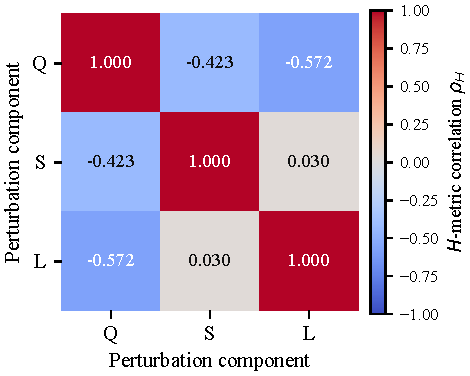
\includegraphics[width=\columnwidth]{figures/hessian_geometry.pdf}
  \caption{Signed activation-Gram correlations for the original conservative
  QSL endpoint, whose natural encoding is tail-padded to the Q+L final byte
  count.  S--L is near zero, while Q--S and Q--L are negative cancellation.
  Scope is one seed and six selected Pythia-70M MLP tensors.}
  \label{fig:geometry}
\end{figure}

\begin{table*}[t]
\centering
\caption{All native endpoints for the three scalability-smoke jobs. Rate and bits/parameter charge complete selected-tensor artifact files. The scopes and tokenizers differ, so rows must only be compared within each model block.}
\label{tab:scaling-pilot-all-endpoints}
\scriptsize
\resizebox{\textwidth}{!}{%
\begin{tabular}{llrrrrrrr}
\toprule
Model & Endpoint & Bytes & Rate & bits/sel. param & $\Delta$NLL & $\Delta$PPL & norm. $H$ & Repair (nnz/rank/dof) \\
\midrule
Pythia-70M & Q & 6,334,784 & 0.2517 & 4.028 & +0.3838 & +43.128 & 0.00961 & 0/0/0 \\
 & Q + global scale & 6,334,784 & 0.2517 & 4.028 & +0.3797 & +42.574 & 0.00946 & 0/0/12 \\
 & Q + block scale & 6,500,672 & 0.2583 & 4.133 & +0.2821 & +30.053 & 0.00597 & 0/0/98304 \\
 & Q+S & 6,520,898 & 0.2591 & 4.146 & +0.2532 & +26.562 & 0.00704 & 27276/0/0 \\
 & Q+S (OBS) & 6,520,898 & 0.2591 & 4.146 & +0.2273 & +23.533 & 0.00611 & 27276/0/27276 \\
 & Q+L & 6,497,344 & 0.2581 & 4.131 & +0.1963 & +19.994 & 0.00476 & 0/30/0 \\
 & Q+S+L strict & 6,497,344 & 0.2581 & 4.131 & +0.2060 & +21.094 & 0.00530 & 5248/16/0 \\
 & Q+S+L strict + scale & 6,497,344 & 0.2581 & 4.131 & +0.2017 & +20.603 & 0.00526 & 5248/16/30 \\
 & Q+S+L relaxed & 6,507,456 & 0.2585 & 4.137 & +0.2028 & +20.733 & 0.00475 & 6470/23/0 \\
 & Q+S (OBS)+L & 6,507,456 & 0.2585 & 4.137 & +0.1988 & +20.276 & 0.00476 & 6470/23/6470 \\
 & Q+S+L relaxed + scale & 6,507,456 & 0.2585 & 4.137 & +0.1993 & +20.333 & 0.00471 & 6470/23/30 \\
\addlinespace
OPT-125M & Q & 11,844,800 & 0.2510 & 4.016 & +0.1295 & +7.744 & 0.00585 & 0/0/0 \\
 & Q + global scale & 11,844,800 & 0.2510 & 4.016 & +0.1163 & +6.913 & 0.00576 & 0/0/10 \\
 & Q + block scale & 12,156,672 & 0.2576 & 4.122 & +0.0604 & +3.491 & 0.00337 & 0/0/175104 \\
 & Q+S & 12,195,064 & 0.2584 & 4.135 & +0.1080 & +6.390 & 0.00420 & 65560/0/0 \\
 & Q+S (OBS) & 12,195,064 & 0.2584 & 4.135 & +0.0999 & +5.884 & 0.00334 & 65560/0/65560 \\
 & Q+L & 12,158,976 & 0.2577 & 4.123 & +0.0735 & +4.272 & 0.00279 & 0/40/0 \\
 & Q+S+L strict & 12,158,976 & 0.2577 & 4.123 & +0.0828 & +4.835 & 0.00309 & 10528/23/0 \\
 & Q+S+L strict + scale & 12,158,976 & 0.2577 & 4.123 & +0.0744 & +4.328 & 0.00307 & 10528/23/30 \\
 & Q+S+L relaxed & 12,201,984 & 0.2586 & 4.138 & +0.0808 & +4.716 & 0.00305 & 13720/27/0 \\
 & Q+S (OBS)+L & 12,201,984 & 0.2586 & 4.138 & +0.0804 & +4.692 & 0.00302 & 13720/27/13720 \\
 & Q+S+L relaxed + scale & 12,201,984 & 0.2586 & 4.138 & +0.0727 & +4.224 & 0.00303 & 13720/27/30 \\
\addlinespace
Qwen3-0.6B & Q & 15,779,648 & 0.2508 & 4.013 & +0.1127 & +3.560 & 0.02295 & 0/0/0 \\
 & Q + global scale & 15,779,648 & 0.2508 & 4.013 & +0.1202 & +3.812 & 0.02204 & 0/0/10 \\
 & Q + block scale & 16,230,272 & 0.2580 & 4.128 & +0.0793 & +2.462 & 0.00662 & 0/0/245760 \\
 & Q+S & 16,254,218 & 0.2583 & 4.134 & +0.0420 & +1.280 & 0.00669 & 95090/0/0 \\
 & Q+S (OBS) & 16,254,218 & 0.2583 & 4.134 & +0.0260 & +0.786 & 0.00386 & 95090/0/95090 \\
 & Q+L & 16,196,352 & 0.2574 & 4.119 & +0.0226 & +0.683 & 0.00414 & 0/50/0 \\
 & Q+S+L strict & 16,196,352 & 0.2574 & 4.119 & +0.0303 & +0.918 & 0.00444 & 17440/30/0 \\
 & Q+S+L strict + scale & 16,196,352 & 0.2574 & 4.119 & +0.0299 & +0.905 & 0.00440 & 17440/30/30 \\
 & Q+S+L relaxed & 16,261,248 & 0.2584 & 4.135 & +0.0224 & +0.676 & 0.00415 & 25458/34/0 \\
 & Q+S (OBS)+L & 16,261,248 & 0.2584 & 4.135 & +0.0224 & +0.675 & 0.00419 & 25458/34/25458 \\
 & Q+S+L relaxed + scale & 16,261,248 & 0.2584 & 4.135 & +0.0219 & +0.660 & 0.00411 & 25458/34/30 \\
\bottomrule
\end{tabular}%
}
\end{table*}


\begin{figure*}[t]
  \centering
  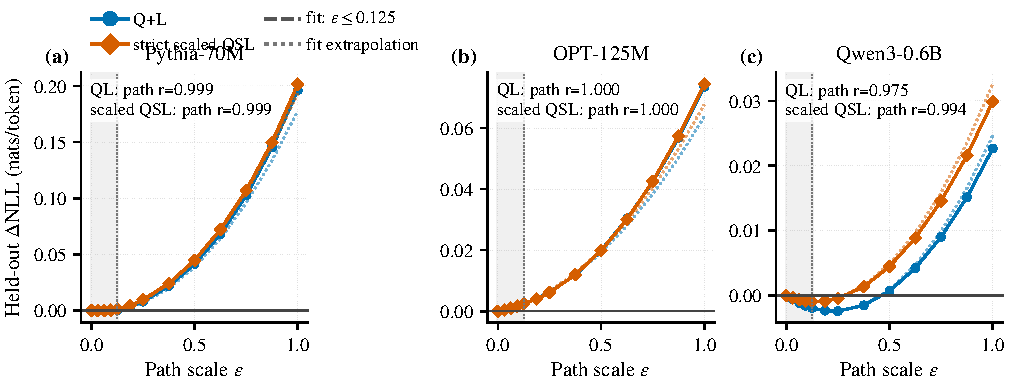
\includegraphics[width=0.99\textwidth]{figures/scaling_pilot_loss_paths.pdf}
  \caption{Thirteen-point one-dimensional interpolation probes for Q+L and
  strict component-scaled QSL in the three separate scalability-smoke jobs.
  Solid points are measured held-out NLL changes.  Dashed curves are fitted
  only on $\epsilon\le0.125$; lighter dotted continuations are extrapolations.
  The shaded region marks the fit interval, and each annotation is the
  path-specific proxy--NLL correlation over 13 points.  Panels use independent
  NLL scales and different tokenizers, so their magnitudes are not compared.
  These slices are not a global loss landscape or multi-seed evidence.}
  \label{fig:scaling-paths}
\end{figure*}


\end{document}
